\documentclass[10pt, oneside]{article}
\usepackage{geometry}             
\geometry{letterpaper, left = 21 mm, right = 21 mm, top = 30 mm, bottom = 25 mm}     


%------------------------macros and packages------------------

%%%Please put path to the downloaded macro file here.
\usepackage{macros} 
%-------------------------begin doc-------------------


\begin{document}

\thispagestyle{empty}
\title{Combinatorial Hypothesis Testing}
\author{Yangxinyu Xie}


%-------------------------------------------------------------------------%

\maketitle
\addtocounter{footnote}{-1}\let\thefootnote\svthefootnote

\section{Introduction}

Suppose we observe an $n$-dimensional vector $\bX = (X_1,...,X_n)$. The null hypothesis $H_0$ is that $\bX \sim \cN(0, \bI)$. We denote the probability measure and expectation under $H_0$ by $\bP_0$ and $\bE_0$, respectively.

Combinatorics kicks in as we consider the alternative hypotheses, by introducing a class $\cC$: consider a class $\cC=\{S_1,\ldots,S_N\}$ of $N$ sets of indices such that $S_k \subset\{1,\ldots,n\}$ and $|S_k| = K$ for all $k=1,\ldots,N$. Under $H_1$, there
exists an $S \in \cC$ such that the distribution of $X_i$ is determined by whether $i$ is in $S$:
\begin{alt}[Detection of Means\cite{arias2008searching, addario2010combinatorial, arias2011detection}]
  \label{alt:mean}
$$
X_i \sim
\begin{cases}
  \cN(0,1), \quad & \mbox{ if }i \notin S\\
  \cN(\mu,1), & \mbox{ if }i \in S
\end{cases}
$$
where $\mu>0$ is a positive parameter and components of $\bX$ are independent. 
\end{alt}
\begin{alt}[Detection of Correlations\cite{arias2012correlation}]
  \label{alt:correlation}
  $X_i \sim \cN(0,1)$ for each $i$ and 
  $$
  \Cov(X_i, X_j) =
  \begin{cases}
    1, \quad & \mbox{ if }i = j\\
    \rho, & \mbox{ if }i \neq j\mbox{ with }i, j \in S\\
    0, & \mbox{ otherwise}\\
  \end{cases}
  $$
  where $\rho \in (0,1).$
\end{alt}

For each $S \in \cC$, we denote the probability measure and expectation by $\bP_S$ and $\bE_S$, respectively. Many interesting combinatorial examples of $\cC$ arises: subsets of size $K$, cliques, perfect matchings, spanning trees, and clusters, etc.

A~\textit{test} is a~binary-valued function $f:\bR^n \to\{
0,1\}$. If
$f(X)=0$, then the test accepts the null hypothesis $H_0$;
otherwise $H_0$ is rejected by $f$.
We measure the performance of a~test based on the \textit{minimax risk}:
\[
R_*^{\max} := \inf_{f} R^{\max}(f).
\]
where $R^{\max}(f)$ is the worst-case risk over the class of interest $\cC$, formally defined by
\[
R^{\max}(f) = \bP_0\{f(X)=1\}
+ \max_{S\in\cC} \bP_S\{f(X)=0\}.
\]

In this report, we discuss the techniques introduced in \cite{arias2012correlation, addario2010combinatorial, arias2011detection} to derive the lower and upper bounds of $R_*^{\max}$, as well as more recent extensions. For a more detailed, yet self-contained, discussion of the proof techniques, we refer the reader to \cite{lugosi2017lectures}.

\section{General Framework}

\subsection{Lower Bounds}
A~standard way to obtain lower bounds for the minimax risk is by putting a~prior on the class $\cC$ and obtaining a~lower bound on the corresponding \textit{Bayesian risk}, which never exceeds the worst-case risk. The
uniform prior on $\cC$ gives rise to the following \textit{average risk}:
\[
R(f) = \bP_0\{f(X)=1\}
+ \bP_1\{f(X)=0\},
\]
where
\[
\bP_1\{f(X)=0\} := \frac{1}{N}\sum_{S\in\cC} \bP_S\{f(X)=0\},
\]
and $N := |\cC|$ is the cardinality of $\cC$.
The advantage of the average risk over the worst-case risk is that the likelihood ratio test, denoted $f^*$, is optimal for the former, according to the Neyman--Pearson lemma. Introducing $L(X)$, the likelihood ratio between $H_0$ and $H_1$, the optimal test becomes
%
\[
f^*(x) = 0  \quad\mbox{if and only if}\quad   L(x) \le 1.
\]
The
%GL
(average)
risk $R^*=R(f^*)$ of the optimal test is called the
\textit{Bayes risk} and it satisfies

\[
R^* = 1 - \frac{1}{2} \bE_0 |L(X) - 1|
\]

\subsection{Upper Bounds}
The analysss of the upper bounds of the risks of optimal tests are often less systematic. Even though likelihood ratio test is optimal in the
Bayesian setting, it is difficult to obtain directly upper bounds for the (worst-case) risk
of the likelihood ratio test. Hence, in analysing combinatorial testing problems, we often focus on obtaining upper bounds for sub-optimal tests for ease of analysis and strive for an upper bound matching the obtained lower bound.


\section{Detection of Means}
In this section we focus on the first alternative hypothesis \ref{alt:mean}. We will first discuss simple tests are considered as we obtain upper bounds: the averaging test and the maximum test. Then, we will provide the key insights driving the results for lower bounds obtained in \cite{addario2010combinatorial} and discuss the applications to examples such as {\bf $k$-sets, spanning trees, perfect matchings, etc}.


\subsection{Upper Bounds}
The \textit{averaging test} has the form
\[
f(\mathbf{x}) = 0  \quad\mbox{if and only if}\quad { \sum_{i=1}^n X_i \le \mu K/2 }.
\]
Since the sum of the components of $\bX$ is zero-mean normal under $\bP_0$
and has mean $\mu K$ under the alternative hypothesis, we obtain the following:
\begin{prop}[\cite{addario2010combinatorial}, Proposition 2.1]
  \label{average}
  Let $\delta>0$. The risk of the averaging test $f$ satisfies
  $R(f) \le\delta$
  whenever
  %
  \[
  \mu\ge\sqrt{\frac{8n}{K^2} \log\frac{2}{\delta}}.
  \]
  %
\end{prop}

The \textit{maximum test} is based on the \textit{scan statistic} $\max_{S\in\cC} X_S$, and it has the form:
%
\[
f(\mathbf{x}) = 0 \quad\mbox{if and only if}\quad
\max_{S\in\cC} X_S\le\frac{\mu K + \mathbb{E}_0 \max_{S\in\cC} X_S}{2}.
\]
Observing that under the alternative hypothesis for some $S\in\cC$, $X_S= \sum_{i\in S} X_i$ is normal
$(\mu K, K)$, we obtain
\begin{prop}[\cite{addario2010combinatorial}, Proposition 2.2]
  \label{maxtest}
  The risk of the maximum test $f$ satisfies
  $R(f) \le\delta$ whenever
  %
  \[
  \mu\ge\frac{\mathbb{E}_0 \max_{S\in\cC} X_S}{K} + 2\sqrt{\frac{2}{K}
  \log
  \frac{2}{\delta}}.
  \]
  %
\end{prop}

{\bf ADD SOMETHING}

\subsection{Lower Bounds}
Let's take a closer look at the likehood ratio. If we write 
\[
\phi_0(\mathbf{x}) = (2\pi)^{-n/2} e^{-\sum_{i=1}^n x_i^2/2} \text{ and }
\phi_S(\mathbf{x}) = (2\pi)^{-n/2} e^{-\sum_{i\in S}(x_i-\mu)^2/2-\sum_{i\notin S} x_i^2/2}
\]
for the
probability densities of $\bP_0$ and $\bP_S$, respectively,
the likelihood ratio at $\mathbf{x}$ is
\[
L(\mathbf{x})
= \frac{{1/N}\sum_{S\in\cC} \phi_S(\mathbf{x})}{\phi
_0(\mathbf{x})}
= \frac{1}{N} \sum_{S\in\cC}
e^{\mu x_S - K\mu^2/2},
\]
where $x_S = \sum_{i\in S} x_i$. With the observation $R^* \ge 1 - \sqrt{1 - (\mathbb{E}_0 \sqrt{L(\bX)})^2}$ (\cite{devroye2013probabilistic}),
we can apply Jensen's inequality, 
\[
\mathbb{E}_0 \sqrt{L(\bX)} = \int\sqrt{\frac{{1/N}\sum_{S\in\cC} \phi_S(\mathbf{x})}{\phi
_0(\mathbf{x})}} \phi
_0(\mathbf{x}) \,d\mathbf{x}
= \int\sqrt{\frac{1}{N} \sum_{S\in\cC} \phi_S(\mathbf{x}) \phi
_0(\mathbf{x})} \,d\mathbf{x}
\ge\frac{1}{N} \sum_{S\in\cC}
\int\sqrt{ \phi_S(\mathbf{x}) \phi_0(\mathbf{x})} \,d\mathbf{x}.
\] 
Because for any $S\in\cC, \int\sqrt{ \phi_S(\mathbf{x}) \phi_0(\mathbf{x})} \,d\mathbf{x}=e^{-\mu^2K/8}$, for all classes $\cC$, $R^* \ge1/2$ whenever
\begin{equation}
  \label{eq: loose lower bound}
  \mu\le\sqrt{(4/K)}\times\sqrt{\log(4/3)}
\end{equation}
i.e. small risk cannot be achieved unless $\mu$ is substantially large compared to $K^{-1/2}$. But this can be substantially improved by the moment method proposed in \cite{addario2010combinatorial}, as we discuss next.

%
\subsubsection{Moment Methods}
\label{subsubsec:Moment Methods}
%

The moment method applies the following insight: by the Cauchy--Schwarz inequality,
%
\[
R^* = 1 - \tfrac{1}{2} \mathbb{E}_0 |L(\bX)-1|
\ge1 - \tfrac{1}{2} \sqrt{\mathbb{E}_0 |L(\bX)-1|^2}.
\]
and since $\mathbb{E}_0 L(\bX) = 1, \mathbb{E}_0 |L(\bX)-1|^2=\Var_0(L(\bX)) = \mathbb{E}_0 [L(\bX)^2] -1.$ 
We are now ready to prove the following lower bound based on overlapping pairs, which reduces the problem to
studying a purely combinatorial quantity \cite{arias2008searching,addario2010combinatorial}:
\begin{prop}[\cite{addario2010combinatorial}, Proposition 3.2]
  \label{prop:pairs}
  Let $S$ and $S'$ be drawn independently, uniformly, at random from $\cC$
  and let $Z=|S\cap S'|$. Then
  \[
  R^* \ge 1- \tfrac{1}{2} \sqrt{\mathbb{E} e^{\mu^2 Z} -1}.
  \]
\end{prop}
\begin{proof}
Because $L(\bX)= \frac1 N \sum_{S\in\cC} e^{\mu X_S -K\mu^2/2}$, 
\[
\mathbb{E}_0 [L(\bX)^2]
=
\frac{1}{N^2} \sum_{S,S'\in\cC} e^{-K \mu^2} \mathbb{E}_0 e^{\mu(X_S+X_{S'})}.
\]
Meanwhile,
\begin{eqnarray*}
\mathbb{E}_0 e^{\mu(X_S+X_{S'})}
& = &
\mathbb{E}_0 [ e^{\mu\sum_{i\in S\setminus S'} X_i} e^{\mu\sum_{i\in
S'\setminus S} X_i}
e^{2\mu\sum_{i\in S\cap S'} X_i} ] \\
& = &
(\mathbb{E}_0 e^{\mu X} )^{2(K-|S\cap S'|)} (\mathbb{E}_0 e^{2\mu X}
)^{|S\cap S'|}
\\
& = &
e^{\mu^2 (K-|S\cap S'|)+2\mu^2|S\cap S'|}
\end{eqnarray*}
\end{proof}

The previous proposition allows us to obtain lower bounds by analysing the quantity $\mathbb{E} e^{\mu^2Z}$. 
This allows us to exploit the combinatorial structures of the class $\cC$ and gives us far better bounds than \ref{eq: loose lower bound}, as the folloiwng examples show:


%\begin{exmp}[Disjoint Sets, \cite{addario2010combinatorial}, Section 4.1]
%  \label{exmp: Disjoint Sets}
%  Suppose all $S\in\cC$ are disjoint (and therefore $KN\le n$). Fix $\delta\in(0,1)$. Let $Z = K$ with probability $1/N$ and $Z = 0$ otherwise. Thus,
%  $$\mathbb{E} e^{\mu^2Z} -1 = \frac{1}{N} (e^{\mu^2 K} -1 )\le\frac{1}{N} e^{\mu^2 K}$$
%  and therefore $R^* \ge\delta$ whenever
%  $$\mu\le\sqrt{\frac{\log(4N(1-\delta)^2)}{K}}.$$
%  Notice that with the bound the bound $\mathbb{E}_0 \max_{S\in\cC} X_S \le\sqrt{2K\log N}$, maximum test $f$ gives us $R^* \le R(f) \le\delta$ whenever
%  $$\mu\ge\sqrt{\frac{2\log N}{K}} + 2\sqrt{\frac{2\log(2/\delta)}{K}}.$$
%  So in this case the critical transition occurs when $\mu$ is of the order of $\hspace*{-0.2pt}\sqrt{(1/K)\hspace*{-0.2pt}\log\hspace*{-0.25pt} N}$.
%\end{exmp}

\begin{exmp}[Spanning Trees, \cite{addario2010combinatorial}, Section 4.5]
  \label{exmp:Spanning Trees}
Let $1,2,\ldots,n={m\choose2}$ represent the edges of the complete graph $K_m$ and let $\cC$ be the set of all spanning trees of $K_m$.
Thus, we have $N=m^{m-2}$ spanning trees and $K=m-1$. With the fact $\mathbb{E}[ e^{\mu^2 Z} ] \le \exp(2e^{\mu^2 })$, we obtain that for any $\delta\in(0,1)$,
$R^* \ge\delta$ whenever
\[
\mu\le\sqrt{\log\bigl(1+\tfrac1 2 \log\bigl(1+4(1-\delta)^2\bigr) \bigr)}.
\]
Meanwhile, the averaging test has risk $R(f) \le\delta$ whenever $\mu\ge\sqrt{4\log(2/\delta)}$.
\end{exmp}

%\begin{exmp}[Cliques, \cite{addario2010combinatorial}, Section 4.6]
%Consider the random variables $X_1,\ldots,X_n$ associated with the edges of the complete graph $K_m$ such that ${m\choose2}=n$ and let $\cC$ contain all cliques of size $k$. Thus, $K={k\choose2}$ and $N={m\choose k}$. With some technical work, one can show that $\mathbb{E}[ \exp(\mu^2Z) ] \le2$. This gives us $R^* \ge1/2$ whenever
%  $$\mu\le\sqrt{\frac{1}{k} \log\biggl(\frac{m}{2k} \biggr)}$$
%Similar to disjoint sets (Example \ref{exmp: Disjoint Sets}), we have with maximum test, $R^* \le\delta$ whenever
%$$\mu\ge O\biggl(\sqrt{\frac{1}{k} \log\biggl(\frac{m}{k} \biggr)}+ \sqrt{\frac{\log(1/\delta)}{k^2}}\biggr)$$
%\end{exmp}

We also explore two special combinatorial structures: \textit{symmetry} and \textit{negative association}.
\begin{defn}[Symmetry]
  \label{defn:symmetry}
  We say that the class $\cC$ is {\it symmetric} if it satisfies the following conditions.
  Let $S,S'$ be drawn independently and uniformly at random from $\cC$. Then,
  \begin{enumerate}
    \item the conditional distribution of $Z=|S\cap S'|$ given $S'$ is identical
    for all values of $S'$;
    \item for any fixed $S_0\in\cC$ and $i\in S_0$, $\bP\{i\in S\}=K/n$.
  \end{enumerate}
\end{defn}
Via H\"older's inequality, we can obtain the following
\begin{prop}[\cite{addario2010combinatorial}, Proposition 3.3]
  \label{prop:symmetric}
  Assume that $\cC$ is symmetric. Then 
  $$\mathbb{E}[ e^{\mu^2 Z}]\le (e^{\mu^2K} -1 ) \frac{K}{n} +1.$$
\end{prop}
%The proposition above shows that for any small and sufficiently symmetric class, the critical value of $\mu$ is of the order of $\sqrt{(\log n)/K}$, at least if $K\le n^\beta$ for some $\beta\in(0,1)$.
%\begin{exmp}[Stars, \cite{addario2010combinatorial}, Section 4.4]
%A star is a subgraph of the complete graph $K_m$ which contains all $K=m-1$ edges incident to a fixed vertex. Consider the set $\cC$ of all stars in $K_m$. In this setting, $n={m\choose2}$ and $N=m$. Hence, for any $\varepsilon>0,$ we have $\lim_{m\to\infty} R^* = 1$ if 
%$$\mu\le(1-\varepsilon)\sqrt{\dfrac{\log m}{m}}$$
%\end{exmp}
\begin{defn}[Negative Association]
  A collection $Y_1,\ldots,Y_n$ of random variables is \textit{negatively associated} if for any pair of disjoint sets $I,J\subset\{1,\ldots,n\}$ and (coordinate-wise) nondecreasing functions $f$ and $g$,
\[
\mathbb{E}[ f(Y_i, i\in I) g(Y_j, j\in J) ]
\le\mathbb{E}[ f(Y_i, i\in I) ] \mathbb{E}[g(Y_j, j\in J) ].
\]
\end{defn}

\begin{prop}[\cite{addario2010combinatorial}, Proposition 3.4]
  \label{negass}
  Assume that the class $\cC$ is symmetric. Suppose that the labels are such that $S'=\{1,2,\ldots,K\} \in\cC$. Let $S$ be a randomly chosen element of $\cC$. If the random variables
  ${\bf 1}_{\{ 1 \in S \}},\ldots,{\bf 1}_{\{ K\in S \}}$ are negatively associated, then 
  $$\mathbb{E}[ e^{\mu^2 Z}]\le \biggl( (e^{\mu^2} -1 ) \frac{K}{n} +1 \biggr)^K.$$
\end{prop}
\begin{exmp}[K-sets, \cite{addario2010combinatorial}, Section 4.2]
  Consider the example when $\cC$ contains all sets $S \subset\{1,\ldots ,n\}$ of size $K$. Note $N={n\choose K}$. This class is symmetric and satisfies the condition in the previous proposition. Hence, applying Proposition \ref{prop:pairs}, $R^*\ge\delta$ for all $\mu$ with
  %
  \[
  \mu\le\sqrt{\log\biggl(1+\frac{n\log(1+4(1-\delta)^2)}{K^2} \biggr)}.
  \]
\end{exmp}
{\bf ADD SOMETHING}

%\begin{exmp}[Perfect Matchings, \cite{addario2010combinatorial}, Section 4.3]
%  \label{exmp:Perfect Matchings}
%  Let $\cC$ be the set of all perfect matchings of the complete bipartite graph $K_{m,m}$. Thus, we have $n=m^2$ edges and $N=m!$, and $K=m$. The symmetry assumptions hold obviously and the negative association property follows from the fact that $Z=|S\cap S'|$ has the same distribution as the number of fixed points in a random permutation. Hence for all $m$, $R^* \ge\delta$ whenever
%$$\mu\le\sqrt{\log\bigl(1+\log\bigl(1+4(1-\delta)^2\bigr)\bigr)}$$
%\end{exmp}

\subsection{Detection of an Anomalous Cluster}
As a special case of the detection of means problem, we can consider the following scenario in network analysis introduced in \cite{arias2011detection}.
Let $\bV_m$ be either derived from a geometric shape or has a graph structure. For simplicity, we can think of $\bV_m$ as the set of graphs with $m$ nodes embedded in the Euclidean space. Let $\Km$ be a class of clusters within $\bV_m$.

Under $H_0^m, \bX \sim \cN(0, \bI_m)$. Under $H_1^m$, there exists a cluster $K \in \Km$ where 
%
\[
X_v \sim\cN(\mu_K,1)\qquad \forall v \in K;\qquad X_v \sim
\cN(0,1)\qquad \forall v \notin K,
\]
%
where $\mu_K > 0$.
We choose to decompose $\mu_K$ as $\mu_K = |K|^{-1/2} \Lambda_K$, where
$|K|$ denotes the number of nodes in $K$ and $\Lambda_K$ is the signal
strength. We say that $H_0^m$ and $H_1^m$ are {\it asymptotically inseparable}
(in the minimax sense) if
%
\[
\liminf_{m \to\infty} R_{*}^{\max} = 1,
\]
%
which is equivalent to saying that, as $m$ becomes large, no test can
perform substantially better than random guessing. A sequence of tests $(T_m)$ is said to {\it asymptotically separate} $H
_0^m$ and $H_1^m$ if
%
\[
\lim_{m \to\infty} R^{\max}(T_m) = 0,
\]

Combining the insight we gained from the moment method earlier and more delicate analysis of the signal $\Lambda_K$, \cite{arias2011detection} shows that if $\Km$ is the set of mild deformations of a unit ball, then under specific conditions,
$H_0^m$ and $H_1^m$ are asymptotically inseparable if there is
$\eta_m \to0$ slowly enough such that, for all $K \in\Km$,
%
\[
\Lambda_K \leq(1 - \eta_m) \sqrt{2 \log(m/|K|)};
\]
%
and conversely, a version of the scan statistic can asymptotically separates $H_0^m$ and $H_1^m$ if there is $\eta_m
\to0$ slowly enough such that, for all $K \in\Km$,
%
\[
\Lambda_K \geq(1 + \eta_m) \sqrt{2 \log(m/|K|)}.
\]
\cite{arias2011detection} also derived bounds for "thin clusters" and paths along a $d$-dimensional lattice. We refer the reader to the orignal paper for details. Notably, the authors also extended their results to exponential families.

\section{Detection of Correlations}
\subsection{Lower Bounds}
First, we note that we can rewrite the alternative hypotheses as $$H_1: \bX \sim\cN(0,\bA_S)\qquad\mbox{for some $S \in\cC$,}$$ where
$$(\bA_S)_{i,j} = \begin{cases}
1, &\quad i = j, \cr
\rho, &\quad i \neq j, i, j \in S, \cr
0, &\quad \text{otherwise}.
\end{cases}$$
Introducing $Z_S = \exp\bigl(\tfrac{1}{2} X^T (\bI- \bA_S^{-1}) X \bigr)$ for all $S \in\cC$, the likelihood ratio between $H_0$ and $H_1$ may be written as $$L(X) = \frac{1}{N} \sum_{S \in\cC} \frac{Z_S}{\bE_0 Z_S}$$ Thus the Bayes risk satisfies
$$R^* = 1 - \frac{1}{2} \bE_0 |L(X) - 1| = 1 - \frac{1}{2} \bE_0\biggl| \frac{1}{N} \sum_{S \in\cC} \frac{Z_S}{\bE_0 Z_S} - 1\biggr|$$

\subsubsection{Generalised Moment Method}
A direct application of the momont method discussed earlier does not yield very promising lowerbounds; instead, we leverage the insight from the folloiwng representation lemma:
\begin{lem}[\cite{berman1962equally};\cite{arias2012correlation}, Lemma 1.1]
  \label{lemrepresent}
  Let $X_1,\ldots, X_k$ be standard normal with $\Cov(X_i, X_j) = \rho
  $ for $i \neq j$. Then there are i.i.d. standard normal random
  variables, denoted $U, U_1,\ldots, U_k$, such that $X_i = \sqrt{\rho}
  U + \sqrt{1-\rho}   U_i$ for all $i$.
\end{lem}
Thus, given $U$, the problem becomes that of detecting a~subset of
variables with nonzero mean (equal to $\sqrt{\rho} U$) and with a~variance equal to $1-\rho$ (instead of 1). We are now ready to reduce analysing testing problem into a combinatorial problem.

\begin{prop}[\cite{arias2012correlation}, Theorem 2.1]
  \label{thmlower}
For any class $\cC$ and any $a~> 0$,
\[
R^* \geq\bP\{|\cN(0,1)| \le a\} \bigl(1 - \tfrac12 \sqrt{\bE
\exp
(\nu_a~Z ) - 1}\bigr),
\]
where $\nu_a~:= \rho a^2/(1+\rho)- \frac12 \log(1-\rho^2)$ and
$Z=|S \cap S'|$, with $S, S'$ drawn independently, uniformly at random
from $\cC$.
\end{prop}

\begin{proof}
  Via Lemma~\ref{lemrepresent}, we can write 
    \[
    X_i = \begin{cases}
    U_i, \quad & \mbox{ if } i \notin S, \cr
    \sqrt{\rho}  U + \sqrt{1-\rho}  U_i, & \mbox{ if } i \in S
    \end{cases}
    \]
  where $U,U_1,\ldots,U_n$ are independent standard normal random variables.
  We consider now the alternative $H_1(u)$, defined as the alternative
$H_1$ given \mbox{$U=u$}.
Let $R(f)$, $L$, $f^*$ [resp., $R_u(f)$, $L_u$, $f_u^*$] be the risk of
a~test $f$, the likelihood ratio, and the optimal (likelihood ratio)
test, for $H_0$ versus $H_1$ [resp., $H_0$~versus $H_1(u)$]. For any $u
\in\bR$, $R_u(f_u^*) \leq R_u(f^*)$, by the optimality of $f_u^*$
for $H_0$ versus $H_1(u)$. Therefore, conditioning on $U$,
$$R^* = R(f^*) = \bE_{U} R_U(f^*) \geq \bE_{U} R_U(f_U^*) = 1 - \tfrac{1}{2} \bE_{U} \bE_0 |L_U(X) - 1|$$
Using the fact that
$\bE_0 |L_u(X) - 1| \le2$ for all $u$, we have
%
\[
\bE_{U} \bE_0 |L_U(X) - 1|
\le2\bP\{|U|>a\} + \bP\{|U|\le a\} \max_{u \in[-a,a]} \bE_0
|L_u(X) - 1|
\]
%
and therefore, using the Cauchy--Schwarz inequality,
%
\begin{eqnarray*}
1 - \frac{1}{2} \bE_{U} \bE_0 |L_U(X) - 1|
& \ge&
\bP\{|U|\le a\}\biggl( 1-\frac{1}{2}\max_{u \in[-a,a]} \bE_0
|L_u(X) - 1|\biggr)
\\
%& \geq& \bP\{|U|\le a\} - \frac12 \max_{u \in[-a,a]} \bE_0 |L_u(X)
%- 1| \\
& \geq& \bP\{|U|\le a\}\biggl(1 - \frac12 \max_{u \in[-a,a]}
\sqrt{\bE_0 L_u^2(X) - 1}\biggr).
\end{eqnarray*}

After some computation, we obtain 
$$\bE_0 L_u^2(X) \le \frac{1}{N^2} \sum_{S, S' \in\cC}
\exp\biggl(\biggl(\frac{\rho u^2}{1+\rho}- \frac12\log(1-\rho
^2)\biggr) |S \cap S'| \biggr)$$
\end{proof}

Again, we reduce the problem to studying the purely combinatorial quantity $Z = |S \cap S'|$. We demonstrate the implications of this proposition via a few examples.
%\begin{exmp}[Disjoint Sets, \cite{arias2012correlation}, Section 2.3.1]
%  Suppose all $S\in\cC$ are disjoint (and therefore $KN\le n$). Let $Z = K$ with probability $1/N$ and $Z = 0$ otherwise. Thus,
%  $$\mathbb{E} e^{\nu Z} -1 = \frac{1}{N} (e^{\nu K} -1)\le\frac{1}{N} e^{\nu K}$$
%  which is bounded by $1$ if $\nu\le\log(N)/k$, in which case $R^* \ge0.3$.
%\end{exmp}

\begin{exmp}[$k$-sets, \cite{arias2012correlation}, Section 2.3.3]
  \label{exmp: k-sets, cor}
  Suppose $\cC$ is the class of all sets of size $k$. By negative association, (see Proposition \ref{negass})
  \[
  \bE e^{\nu Z} \le\biggl((e^\nu-1) \frac{k}{n}+1\biggr)^k
  \le\exp\biggl((e^\nu-1) \frac{k^2}{n}\biggr),
  \]
  which implies that $R^* \to1$ if either $k^2/n \to\infty$ and $\rho k^2/n \to0$, or $(1-\rho)n^2/k^4 \to\infty$.
\end{exmp}

%\begin{exmp}[Perfect Matchings, \cite{arias2012correlation}, Section 2.3.4]
%  Suppose $\cC$ is the class of all perfect matchings of size $k = \sqrt{n}$. Using the same $Z$ as in Example \ref{exmp:Perfect Matchings},
%  $$\bE e^{\nu Z} \le\biggl((e^\nu-1) \frac{k}{n}+1\biggr)^k\le\exp\biggl((e^\nu-1) \frac{k^2}{n}\biggr),$$
%  which is bounded by 2 when 
%  $$\frac{k^2}{n} \le\frac{\ln2}{\exp(\nu(\rho)) -1}$$
%  in which case $R^* \ge0.3$.
%\end{exmp}

\begin{exmp}[Spanning Trees, \cite{arias2012correlation}, Section 2.3.5]
  Suppose $\cC$ is the class of all spanning trees of a complete graph with $k+1$ vertices. Similar to Example \ref{exmp:Spanning Trees}, notice
  \[
  \bE e^{\nu Z} \le \exp{2(e^\nu-1)},
  \]
  which implies that $R^* \to1$ if $\rho\to0$.
\end{exmp}


\subsection{Upper Bounds}

The \textit{squared-sum test} is based on the observation that under $\bP_0$, $(\sum_{i=1}^n X_i)^2$ is distributed as $n
\chi_1^2$, while for
any $S\subset\{1,\ldots,n\}$ with $|S|=k$, under
$\bP_S$, $(\sum_{i=1}^n X_i)^2$ has the same distribution
as $(n + \rho k(k-1)) \chi_1^2$. This implies that the squared-sum test is near-optimal for detecting
$k$-sets in the regime where $k^2/n \to\infty$, as stated in the following proposition.
%
%pr3.1 #&#
\begin{prop}[\cite{arias2012correlation}, Proposition 3.1]
\label{prpsq}
Let $\cC$ be an arbitrary class of sets of size $k$ and suppose that $\rho k^2/n \to\infty$.
If $t_n$ is such that $t_n\to\infty$ but $t_n = o(\rho k^2/n)$, then the test which rejects the null hypothesis
if $(\sum_{i=1}^n X_i)^2 > n t_n$ has a~worst-case risk converging to zero.
\end{prop}
Notice that in this case, i.e. $k^2/n \to\infty$, Example \ref{exmp: k-sets, cor} implies that any test based on $(\sum_{i=1}^n X_i)^2$ is powerless if $\rho k^2/n \to0$.

The \textit{generalized likelihood ratio test} (GLRT) has the form
%
\[
f(X)=0  \quad\mbox{if and only if}\quad
\max_{S \in\cC} X^T (\bI- \bA_S^{-1}) X \leq t
\]
%
for some appropriately chosen $t$. This is based on the folloiwng observation:
under $\bP_0$, $X^T (\bI- \bA_S^{-1}) X$ is distributed as
%
\[
- \frac{\rho}{1-\rho} \chi^2_{k-1} + \frac{\rho(k-1)}{1 + \rho(k-1)} \chi^2_1,
\]
%
and under the alternative $\bP_S$, it has the same distribution as
%
\[
-\rho\chi^2_{k-1} + \rho(k-1) \chi^2_{1},
\]
%
where $\chi_1^2$ and $\chi_{k-1}^2$ denote independent $\chi^2$
random variables with degrees of freedom $1$ and $k-1$, respectively. Careful analysis based on this observation gives us the folloiwng result:

\begin{prop}[\cite{arias2012correlation}, Proposition 3.3] \label{prpglrt-large}
Consider a~class $\cC$ of sets of size $k$, with cardinality $N \to
\infty$ such that $\log(N)/k
\to\infty$. When $\eta:= (1-\rho) N^{2/k} (\log N)/k \to0$, the
generalized likelihood
ratio test with threshold value $t = -(\log N)/\sqrt{\eta}$ has
worst-case
risk tending to zero.
\end{prop}

Notice that in Proposition~\ref{prpglrt-large} the condition on $\rho
$ implies
that $\rho\to1$, which is much stronger than what the squared-sum
test requires when $k^2/n \to\infty$.
For $k$-sets, $N = {n \choose k}$---so that $\log N = k \log(n/k) +
O(k)$---and the requirement is that $(1-\rho) (n/k)^2 \log(n/k) \to
0$, which is substantially stronger than what the lower bound obtained
in Example \ref{exmp: k-sets, cor} requires. In fact, if $\rho$ is bounded away from 1, then the GLRT may be powerless (\cite{arias2012correlation}, Theorem 3.1).


The \textit{goodness of fit test} (GOF test) is based on the folloiwng insight.
Let $H_i = \Phi^{-1}(X_i)$, where $\Phi$ is the standard normal distribution
function. Under the null, the $H_i$'s are i.i.d. uniform in $(0,1)$.
Under an alternative with anomalous set denoted by $S$, the $X_i, i
\in S$ are closer together, especially since we place ourselves in the
regime where $\rho\to1$. More precisely, we have the following.
%
%le3.1 #&#
\begin{lem} \label{lemclose}
Suppose $X_1,\ldots, X_k$ are
%GL standardized
zero-mean, unit-variance
random variables satisfying $\Cov(X_i, X_j) \geq\rho> 0$, for all $i
\neq j$. Let $\overline{X}$ denote their average. Then for any $t > 0$,
%
\[
\bP\bigl\{ \# \{i: |X_i - \overline{X}| > t\} \geq k/2\bigr\}
\leq\frac{2(1-\rho)}{t^2}.
\]
%
\end{lem}

Choose an integer $m$ such that $m \gg(n/k^2) \log(n/k^2)$ and partition
the interval $[0,1]$ into $m$ bins of length $1/m$, denoted $I_s,  s =
1,\ldots, m$. Let $B_s = \# \{i: H_i \in I_s\}$ be the bin
counts---thus, we are computing a~histogram. Then consider the
following GOF test:
%
\[
f(X)=0  \quad\mbox{if and only if}\quad
\max_{s = 1,\ldots, m} B_s \leq t,
\]
%
where $t$ is some threshold. The folloiwng result suggests that, ignoring logarithmic factors, the GOF test is near-optimal for detecting $k$-sets in
the regime where $k^2/n \to0$ and $k/\log n \to\infty$.

\begin{prop} \label{prpgof}
Consider the class $\cC$ of all $k$-sets in the case where $k^2/n \to
0$ and $k/\log n \to\infty$. In the GOF test above, choose $m$ such
that $(n/k^2) \log n \ll m \ll n/\log n$. When $(1-\rho)^{1/2} \ll
1/m$, the resulting test with threshold $t = n/m + \sqrt{3 n \log(m)/m}$ has
worst-case risk tending to zero.
\end{prop}

{\bf WRITE A SUMMARY}

\section{Extension}

Subsequent lines of work have found more settings where the moment methods introduced in earlier sections can be systematically applied to derive minimax lower bounds for testing problems. In this section, we focus on introducing these scenarios. 
On the other hand, as mentioned earlier, the upper bounds are more often obtained by considering different proposed tests, whose analyses are often much more delicate. Hence, we refer the reader to the respective papers for analyses for the upper bounds.

\subsection{Dectection of positive correlations in a multivariate sample}
A direct extension of the dectection of correlation problem is considered in \cite{arias2015correlations}. Under the alternatives, we make a slight modification of the alternative hypotheses \ref{alt:correlation}, which is, if $i \ne j, i,j \in S$, we have $\Cov(X_i, X_j) \ge \rho > 0$.  the covariance matrix is still sparse, i.e., $k < n/2$ or $k = o(n)$, meaning that only a few variables are substantially correlated. Examples of this setting includes the block model, cliques and perfect matchings. 

Via a more delicate version of the generalized moment method we saw, we can obtain the following:
\begin{prop}[\cite{arias2015correlations}, Theorem 1]
  For any class $\cC$, any $\rho\in(0, 1)$, and any $a \ge\sqrt{3}$,
  \begin{equation}
  \label{lower} R^* \geq\bP \bigl(\chi_m^2 \le m
  a^2 \bigr) \biggl(1 - \frac{1}2 \sqrt{\bE\min \bigl[\exp (m
  \nu_a Z ), \cosh^m(\xi_a Z) \bigr] - 1}
  \biggr),
  \end{equation}
  %
  where
  %
  \[
  \nu_a := \frac{\rho a^2}{1+\rho} - \frac{1}2 \log\bigl(1-
  \rho^2\bigr)\quad  \mbox{and}\quad  \xi_a := \frac{\rho a^2}{1-\rho^2},
  \]
  %
  and where $\chi_m^2$ has chi-squared distribution with $m$ degrees of
  freedom, and $Z=|S \cap S'|$ with $S, S'$ i.i.d. uniform from $\cC$.
\end{prop}
The upper bounds are obtained via squared-sum test and "localized" squared-sum test. 

\subsection{Dectection of sparse principal components of a high-dimensional covariance matrix}
Introduced in \cite{berthet2013optimal}, we can consider the alternative hypothesis $\bX \sim \cN(0, \bI + \theta v v^T)$ where $\theta >0$ and $v$ is $k$-sparse. The techniques for proving the minimax lower bound is much more technical and involves studying the $\chi^2$ distance between probability measures. Yet, the moment methods still palys a key role in showing the following result:
\begin{prop}[\cite{berthet2013optimal}, Theorem 5.1]
  Fix $\nu > 0$. There exists a constant $C_{\nu}$ such that if 
  $$\theta < \min(\sqrt{\frac{k \log(C_{\nu}p/k^2 + 1)}{n}}, \frac{1}{\sqrt{2}})$$
  Then
  $R^* \ge 0.5 - \nu$.
\end{prop}

\subsection{Combinatorial inference for graphical models}

More recently, \cite{neykov2019combinatorial} introduced a new family of combinatorial inference problems for graphical models. Unlike classical statistical inference where the main interest is point estimation or parameter testing, combinatorial inference aims at testing the global structure of the underlying graph. Examples include testing the graph connectivity, the presence of a cycle of certain size, or the maximum degree of the graph.

\section{More Examples}

In this section we introduce two examples that do necessarily satisfy symmetry or negative association. Although it is not immediate what applications these examples can lead to, they may inspire other novel tools to study combinatorial testing problems.

\subsection{Paths on a tree}
Consider a full binary tree whose depth is equal to $m$. Then there are $n = 2m-2$ edges on this tree. Let $\cC$ be the class of all possible paths from the root node to a leaf. Then $N = |\cC| = 2^m$ and for each $S \in \cC, K = m$. 

Notice that this class does not satisfy the second conditon of symmetry in Definition \ref{defn:symmetry}. Because for a fixed path $S_0 \in \cC$, the probability that an edge on $S_0$ at depth $i$ is in another uniformly random path $S$ is $\bP(i \in S) = 2^{-i}.$ Neither are this random variables ${\bf 1}(i \in S)$ negatively associated: for example, the second edge on $S_0$ is in $S$ only if the first edge is in $S$ already, i.e.
$$\bP(1 \in S, 2 \in S) = \bP(2 \in S) >\bP(1 \in S)\bP(2 \in S) $$

The first condition of symmetry still holds, which makes it possible to modify Proposition \ref{prop:symmetric} to obtain a bound. However, in this case, we can compute the moment generating function exactly since $Z$ is geometrically distributed with $p = 1/2.$
$$\bE[e^{\nu Z}] = \frac{p e^{\nu Z}}{1 - (1-p)e^{\nu Z}} = \frac{2}{2 - e^{\nu Z}} - 1$$
By Proposition \ref{prop:pairs}, with $\nu = \mu^2$, we obtain that for any $\delta\in(0,1)$, $R^* \ge\delta$ whenever
$$\mu\le\sqrt{\log\bigl(2-\frac{1}{2(1-\delta)^2 + 1}\bigr)}.$$
By Proposition \ref{thmlower}, with $\nu = \nu_a$, we obtain as $\rho \to 0$, $\nu_a \to 0$, thus $\bE[e^{\nu Z}] \to 1$ and $R^* \to 1$.

\subsection{Triangulations on a k-gon and Catalan Numbers}
Consider a convex $m$-gon, $m \ge 5$. We describe the class $\cC$ as follows. Let $G$ be a complete graph whose $m$ vertices are embedded on a convex $m$-gon. Let $1,...,n$ index the edges in $E(G)\setminus E(\partial G)$; that is, $1,..., n = m(m-1) - m = (m-1)^2$ are the edges in the interior of this $m$-gon. Let $S$ be the set of interior edges of a non-intersecting triangulation of this $m$-gon and let $\cC$ contain all sets of this form. Then,
$K = |S| = m - 3$ and $N = c(m-2)$, where $$c(n) = \frac{1}{n+1}\binom{2n}{n}$$
is the Catalan number. This class does not satisfy the first condition of symmetry. To see this, consider the case of hexagon shown below:\\
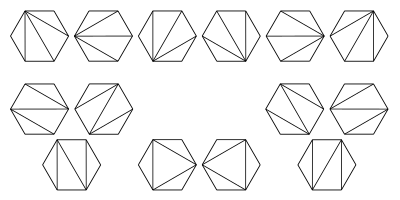
\includegraphics{hexagon.png}\\
Let $S'$ be the triangulation on the upper left corner. Then we have 
$$\bP(Z = 0|S') = 5/14, \bP(Z = 1|S') = 5/14, \bP(Z = 2|S') = 3/14, \bP(Z = 3|S') = 1/14$$
Meanwhile, let $S''$ be the triangulation on the second to last one on lower right corner, whose three interior edges forms a triangle. In this case,
$$\bP(Z = 0|S'') = 4/14, \bP(Z = 1|S'') = 6/14, \bP(Z = 2|S'') = 3/14, \bP(Z = 3|S'') = 1/14$$
Neither does this class satisfy negative association. Intuitively, if one edge comes us in a uniform triangulation, then the edges not interesting with this one will more likely show up in this random triangulation. For example, let $S'$ be the first triangulation in the upper left corder and let $1$ denote the vertical edge and $2$ the diagonal edge. Then
$$\bP(1 \in S, 2 \in S) = \frac{2}{14} > \frac{5}{14} \times \frac{4}{14} = \bP(1 \in S)\bP(2 \in S) $$
It is less clear how to can bound the moment generating function of $Z$ in this case. Hence, deeper understanding of the combinatorial structure of this set will be helpful.

Catalan numbers is a recurrent theme in combinatorics. It counts the number of binary trees, plane trees, ballot sequences, parenthesizations, and Dyck paths, to just name a few examples \cite{stanley2015catalan}. The omnipresence of Catalan numbers allows us to understand many combinatorial classes simultaneously. Hence, it is an interesting future direction to understand the moment generating function of the Catalan-type class and study the testing problem for some of the combinatorial classes of this family. 
\bibliographystyle{plain}
\bibliography{bibfile}
\end{document}
